\begin{frame}[parent={ie:agenda}, hasnext=true, hasprev=false]
	\frametitle{MPS.BR}
	
	\begin{block:concept}{Objetivo}
		Melhoria de processos de software nas micros, pequenas e médias empresas
		(PMEs), a um custo acessível, em diversos locais do país.
	\end{block:concept}
	
	\begin{block:fact}{}
		\begin{itemize}
			\item CMMi + ISO 15504 + ISO 12207
			\item Softex + Governo + universidades
		\end{itemize}
	\end{block:fact}
\end{frame}


\begin{frame}[hasnext=true, hasprev=true]
	\frametitle{MPS.BR}
	
	\begin{block:fact}{Base técnica}
		\centering
		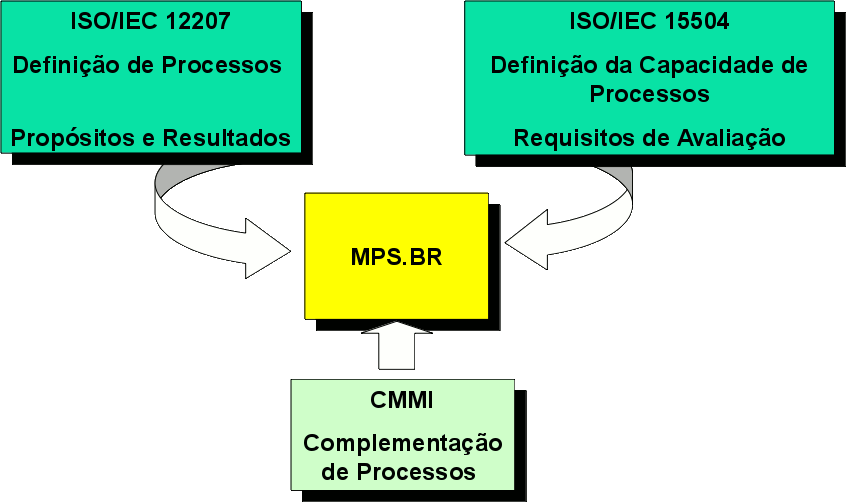
\includegraphics[width=\textwidth]{software-engineering/project-management/process/process-quality/mpsbr/technical-base}
	\end{block:fact}
\end{frame}


\begin{frame}
	\frametitle{MPS.BR}
	
	\begin{block:fact}{Estrutura}
		\centering
		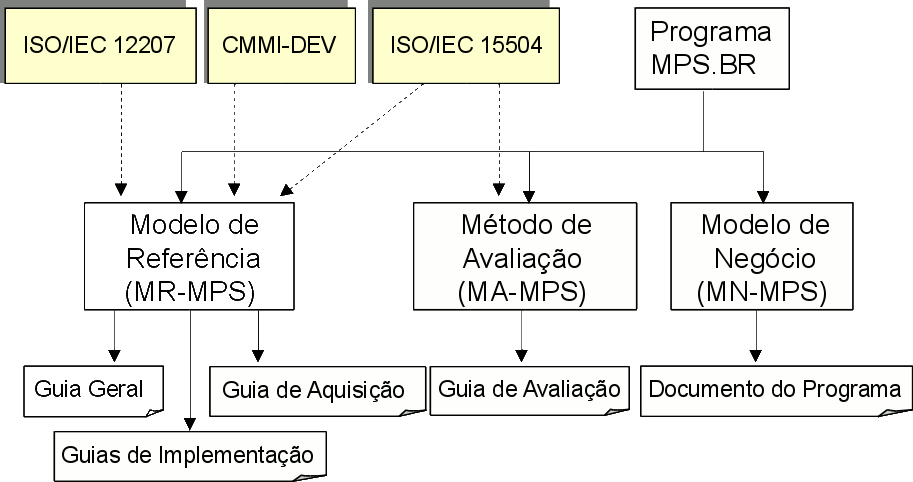
\includegraphics[width=\textwidth]{software-engineering/project-management/process/process-quality/mpsbr/structure}
	\end{block:fact}
\end{frame}



\begin{frame}
	\frametitle{MPS.BR}
	\framesubtitle{Guia geral}
	
	\begin{block:concept}{Guia geral}
		Descreve o Modelo de Referência para Melhoria de Processo de Software
		(MR-MPS)
	\end{block:concept}

	\begin{block:fact}{Características}
		\begin{itemize}
			\item Níveis de maturidade
			
			\item Processos
			\begin{itemize}
				\item Propósitos
				\item Resultados esperados
			\end{itemize}
			
			\item Atributos de processo
			\begin{itemize}
				\item Resultados esperados
			\end{itemize}
		\end{itemize}
	\end{block:fact}
	
	\note{
		As atividades e tarefas necessárias para atender aos propósitos e obter os
		resultados esperados de um processo não são definidos!
	}
\end{frame}



\begin{frame}
	\frametitle{MPS.BR}
	\framesubtitle{Níveis de maturidade}
	
	\begin{block:fact}{Níveis de maturidade}
		\centering
		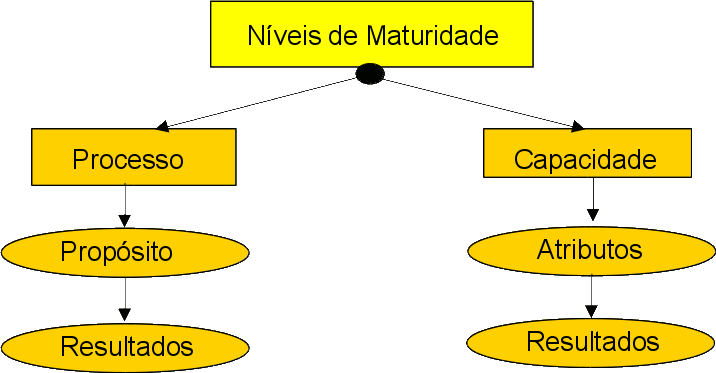
\includegraphics[width=\textwidth]{software-engineering/project-management/process/process-quality/mpsbr/maturity-level}
	\end{block:fact}
\end{frame}



\begin{frame}
	\frametitle{MPS.BR}
	\framesubtitle{Níveis de maturidade}
	
	\begin{block:fact}{Níveis}
		\begin{itemize}
			\item A (em otimização)
			\item B (gerenciado quantitativamente)
			\item C (definido)
			\item D (largamente definido)
			\item E (parcialmente definido)
			\item F (gerenciado)
			\item G (parcialmente gerenciado)
		\end{itemize}
	\end{block:fact}
\end{frame}


\begin{frame}
	\frametitle{MPS.BR}
	\framesubtitle{Níveis de maturidade}
	
	\begin{block:fact}{Níveis de maturidade e processos}
		\centering
		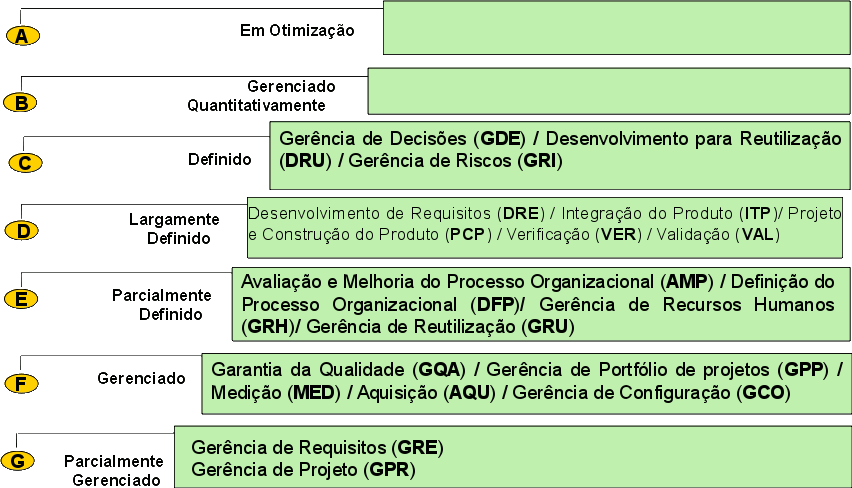
\includegraphics[width=\textwidth]{software-engineering/project-management/process/process-quality/mpsbr/levels-processes}
	\end{block:fact}
\end{frame}


\begin{frame}
	\frametitle{MPS.BR}
	\framesubtitle{Níveis de maturidade}
	
	\begin{block:concept}{Capacidade de processo}
		Expressa o grau de refinamento e institucionalização com que o processo é
		executado na organização ou unidade organizacional, grau este medido pelo
		atendimento de atributos de processo.
	\end{block:concept}

	\begin{block:fact}{Atributos de processo}
		\begin{itemize}
			\item AP 1.1 -- processo é executado
			\item AP 2.1 -- processo é gerenciado
			\item AP 2.2 -- produtos de trabalho do processo são gerenciados
			\item AP 3.1 -- processo é definido
			\item AP 3.2 -- processo está implementado
			\item AP 4.1 -- processo é medido
			\item AP 4.2 -- processo é controlado
			\item AP 5.1 -- processo é objeto de inovações
			\item AP 5.2 -- O processo é otimizado continuamente
		\end{itemize}
	\end{block:fact}
	
	\note{
		\begin{itemize}
			\item Está relacionada com o atendimento aos atributos de processo (AP)
			associados aos processos de cada nível de maturidade.
			\item Cada AP está relacionado com um conjunto de resultados esperados de
			atributo de processo (RAP).
		\end{itemize}
	}
\end{frame}


\begin{frame}
	\frametitle{MPS.BR}
	\framesubtitle{Níveis de maturidade}
	
	\begin{block:fact}{Atributos de processo e resultados esperados}
		Cada AP está relacionado com um conjunto de resultados esperados de atributo de processo (RAP).
	\end{block:fact}
	
	\begin{block:fact}{Exemplo de AP - RAP}
		\begin{itemize}
			\item AP 1.1 -- Processo é executado
			\begin{itemize}
				\item RAP 1. O processo atinge seus resultados definidos
			\end{itemize}
	
			\item AP 2.1 – O processo é gerenciado
			\begin{itemize}
				\item RAP 2. Existe uma política organizacional estabelecida e mantida
				para o processo.
				\item RAP 3. A execução do processo é planejada.
			\end{itemize}
		\end{itemize}
	\end{block:fact}
\end{frame}


\begin{frame}
	\frametitle{MPS.BR}
	\framesubtitle{Níveis de maturidade, processos e capacidades}
	
	\begin{block:fact}{}
		\centering
		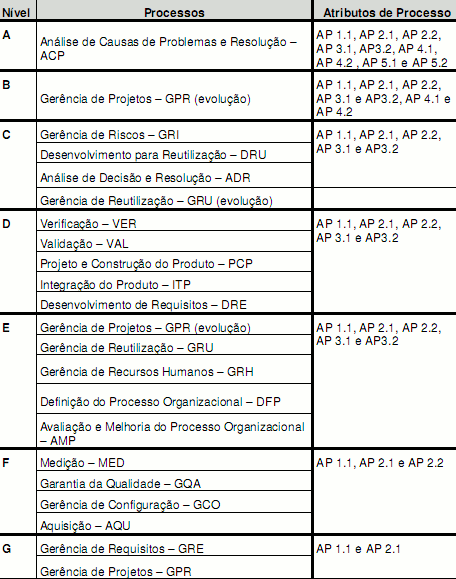
\includegraphics[width=.6\textwidth]{software-engineering/project-management/process/process-quality/mpsbr/levels-processes-capacities}
	\end{block:fact}
\end{frame}


\begin{frame}
	\frametitle{MPS.BR}
	\framesubtitle{Guia geral. Nível G. Gerência de Projetos}
	
	\begin{block:concept}{Propósito}
		Estabelecer e manter planos que e definem atividades, recursos e
		responsabilidades do projeto e que forneçam informações sobre o 
		andamento do projeto que permitam a realização de correções quando houver
		desvios significativos no desempenho. 
	\end{block:concept}

	\begin{block:fact}{Resultados esperados}
		\small
		\begin{itemize}
			\item GPR 1. O escopo do trabalho para o projeto é definido
			\item GPR 2. As tarefas e os produtos do projeto são dimensionados
			utilizando métodos apropriados
			\item GPR 3. O modelo e as fases do ciclo de vida do projeto são
			definidos
			\item GPR 4. (Até o nível F) O esforço e o custo para a execução das
			tarefas e dos produtos de trabalho são estimados com base em dados
			histórios ou referências técnicas
			\item \ldots
		\end{itemize}
	\end{block:fact}
\end{frame}



\begin{frame}
	\frametitle{MPS.BR}
	\framesubtitle{Guia geral. Nível G. Gerência de Projetos}
	
	\begin{block:fact}{Nível G}
		\centering
		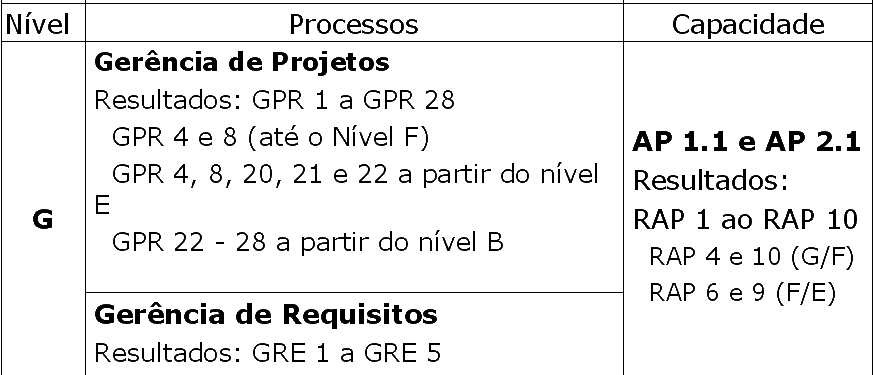
\includegraphics[width=\textwidth]{software-engineering/project-management/process/process-quality/mpsbr/mpsbr-level-g}
	\end{block:fact}
\end{frame}



\begin{frame}
	\frametitle{MPS.BR}
	\framesubtitle{Avaliação}
	
	\begin{block:procedure}{Passos para caracterização de nível}
		\begin{enumerate}
			\item Caracterizar o grau de implementação de cada resultado esperado do
			processo e de cada resultado de atributo de processo \textbf{em cada projeto}
		
			\item Caracterizar inicialmente o grau de implementação de cada resultado
			esperado do processo e de cada resultado de atributo do processo \textbf{na UO}
		
			\item Caracterizar inicialmente o grau de implementação de cada atributo de
			processo \textbf{na UO}

			\item Caracterizar o grau de implementação dos processos \textbf{na UO}

			\item Atribuir nível MPS.BR.
		\end{enumerate}
	\end{block:procedure}
\end{frame}


\begin{frame}
	\frametitle{MPS.BR}
	\framesubtitle{Grau de implementação}
	
	\begin{block:fact}{Caracterização do resultado esperado de processos e
	atributos em cada projeto}
		\centering
		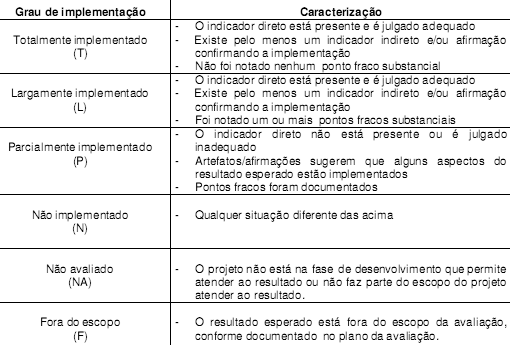
\includegraphics[width=.95\textwidth]{software-engineering/project-management/process/process-quality/mpsbr/mpsbr-implementation-ratings}
	\end{block:fact}
\end{frame}



\begin{frame}
	\frametitle{MPS.BR}
	\framesubtitle{Grau de implementação}
	
	\begin{block:fact}{Caracterização do resultado esperado de processos e
	atributos na UO}
		\centering
		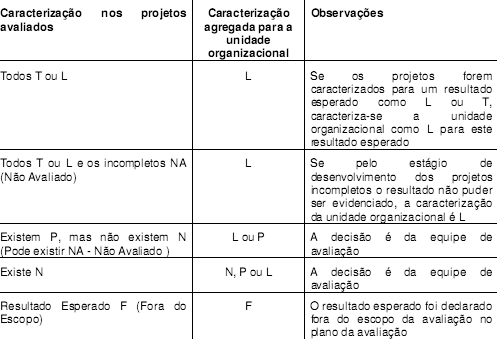
\includegraphics[width=.95\textwidth]{software-engineering/project-management/process/process-quality/mpsbr/mpsbr-implementation-ratings-uo}
	\end{block:fact}
\end{frame}


\begin{frame}
	\frametitle{MPS.BR}
	\framesubtitle{Grau de implementação}
	
	\begin{block:fact}{Caracterização do resultado esperado de atributos na UO}
		\centering
		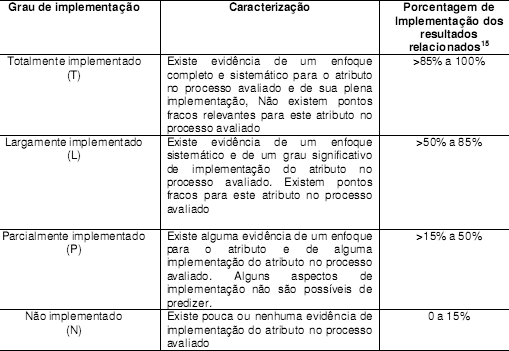
\includegraphics[width=\textwidth]{software-engineering/project-management/process/process-quality/mpsbr/mpsbr-attribute-ratings-uo}
	\end{block:fact}
\end{frame}



\begin{frame}
	\frametitle{MPS.BR}
	\framesubtitle{Grau de implementação}
	
	\begin{block:fact}{Caracterização do nível}
		Um processo está SATISFEITO quando:
		\begin{itemize}
			\item Todos os resultados esperados para o processo foram caracterizados
			como T (Totalmente Implementado) ou L (Largamente Implementado).
			
			\item Tem-se resultados para os atributos do processo, conforme a tabela
			apresentada.
		\end{itemize}
	\end{block:fact}
\end{frame}

\begin{frame}
	\frametitle{MPS.BR}
	\framesubtitle{Grau de implementação}
	
	\begin{block:fact}{Caracterização do nível}
		\centering
		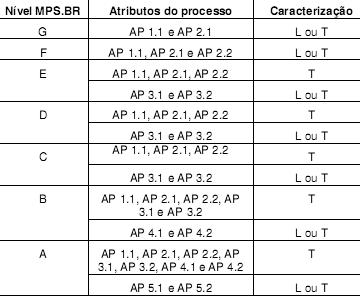
\includegraphics[width=.85\textwidth]{software-engineering/project-management/process/process-quality/mpsbr/mpsbr-ratings-uo}
	\end{block:fact}
\end{frame}


\begin{frame}
	\frametitle{MPS.BR}
	\framesubtitle{Considerações finais}
	
	\begin{block:fact}{Diferenciais}
		\begin{itemize}
			\item 7 níveis de maturidade
			\begin{itemize}
				\item implantação mais gradual
				\item maior visibilidade dos resultados de melhoria de processo
				\item prazos mais curtos
			\end{itemize}
			
			\item Compatibilidade com CMMI, conformidade com as normas ISO/IEC 15504
			e 12207.
			
			\item Adaptado para a realidade brasileira (foco em micro, pequenas e
			médias empresas).
			
			\item Custo acessível (em R\$)
		\end{itemize}
	\end{block:fact}
\end{frame}



\begin{frame}
	\frametitle{MPS.BR}
	\framesubtitle{Considerações finais}
	
	\begin{block:fact}{MPS.BR e CMMi}
		\centering
		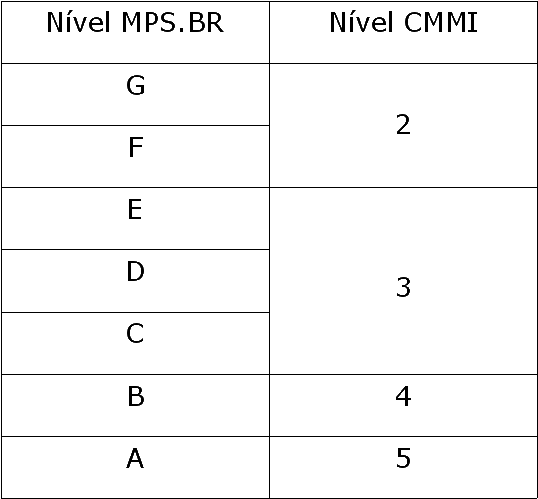
\includegraphics[width=.7\textwidth]{software-engineering/project-management/process/process-quality/mpsbr/mpsbr-cmmi}
	\end{block:fact}
\end{frame}